\documentclass{article}
\usepackage[english]{babel}
\usepackage[a4paper,top=2cm,bottom=2cm,left=3cm,right=3cm,marginparwidth=1.75cm]{geometry}

% Packages
\usepackage{amsmath}
\usepackage{tikz}
\usepackage{caption}
\usepackage{algorithm}
\usepackage{algpseudocode}
\usepackage{pgfplots}
\pgfplotsset{width=10cm,compat=1.9}

\tikzset{
  treenode/.style = {align=center, circle, black, inner sep=0pt, text centered,
    font=\sffamily, draw=black, text width=1.5em, very thick}
}

\newcommand\catalannumber[4]{
  % size, path (list of integers), offset
  \fill[cyan!25]  (0,- #1 - 1) rectangle +(#2,#1);
  \draw (0, - #1 -1) grid +(#2,#1);
  
  \draw[dashed] (0,-#1 - 1 + #4) -- +(#1 - #4,#1 - #4);
  \coordinate (prev) at (0, - #1 -1);
  \foreach \dir in {#3}{
    \ifnum\dir=0
    \coordinate (dep) at (1,0);
    \else
        \ifnum\dir=1
        \coordinate (dep) at (0,1);
        \else
            \ifnum\dir=2
            \coordinate (dep) at (-1,0);
            \else
            \coordinate (dep) at (0,-1);
            \fi
        \fi
    \fi
    \draw[line width=2pt,-stealth,red] (prev) -- ++(dep) coordinate (prev);
  };
}

\newcommand\catalannumberextended[4]{
  % size, path (list of integers), offset
  \fill[cyan!25]  (0,- #1 - 1) rectangle +(#1 - 1 - #4, #1 + 1);
  \draw[dotted] (0, - #1 -1) grid +(#1 - 1 - #4,#1 + 1);
  
  \catalannumber{#1}{#2}{#3}{#4}
}

\title{Succinct data structures for generalized rank/select queries on lists of integers and their use for representing sequences of balanced parenthesis}
\author{Fabrizio Brioni}

\begin{document}
\maketitle

\begin{abstract}
This document will describe a succinct data structure for generalized rank/select queries on lists of integers. Initially it will be defined a generalization of the classical operations of rank and select on sequences of bits. Then the segment tree data structure will be described, followed by a description of a two-level organization (similar to the Jacobson rank structure) for storing information about lists of integers and then an explanation of how to integrate the two structures to handle generalized rank/select queries efficiently and succinctly.
\end{abstract}

\section{Introduction}
Let $v$ be a sequence of bits of length $n$ numbered from $0$ to $n-1$ and $v_i$ the $i$-th bit of $v$, rank and select queries are usually defined as follows:
    \begin{itemize}
        \item $\text{rank}_v(i)$ is the number of bits equal to 1 preceding the i-th bit:
            $$\text{rank}_v(i)=|\{j : j<i \land v_j=1\}|;$$
        \item $\text{select}_v(i)$ is the index of the ($i+1$)-th bit equal to 1 in the sequence if it exists, otherwise it is equal to $n$:
            $$\text{select}_v(i)=\max\{j : \text{rank}(j) \leq i \land j \leq n\}.$$ 
    \end{itemize}
Now consider a list of $n$ integers between $-M$ and $M$, the information-theoretic lower bound for its representation will be $\log{((2M+1)^n)}=n\log{(2M+1)}$.
In this document will be defined a possible extension of rank/select queries suitable on lists of integers and devised a succinct data structure that, given an integer list of length $n$, implements such operations with a time complexity of $\mathcal{O}(\log{n})$ using $n\log{(2M+1)} + o(n\log{(2M)})$ bits of memory. Also it will be shown how a possible use of such generalized rank/select queries is the management of sequences of balanced parentheses.

\section{Notations}
Let $v$ be a list of $n$ integers numbered from $0$ to $n-1$ and $v_i$ the integer with index $i$. We define the generalized rank query as
    $$\mathit{rank}_v(i)=\sum_{i=0}^{i-1}v_i$$
that is the sum of the integers with index less than $i$. In this way the formal definition of a select operation can remain the same as the classical one, that is
    $$\mathit{select}_v(i)=\max\{j : \mathit{rank}_v(j) \leq i \land j \leq n\}$$
but it has another meaning: $\text{select}_v(i)$ is equal to the maximum prefix of $v$ with sum less than or equal to $i$. However, this operation of select is not enough to operate on a list of integers, because in a list $v$ of integers (of which some negatives) there can be two indexes $i < j$ (or more than two) with $\text{rank}_v(i) = \text{rank}_v(j)$ and in that case the index $i$ will never be the result of a select query (which will always prefer $j$ or a possible subsequent index). Then it may be useful to add an argument to the select query so that you can control the portion of the list that is being examined and so that each index may be the result of a select query. This results in the following definition of generalized select:
    \begin{align*}
        \mathit{selectLast}_v(i,u)=
            \begin{cases}
                \max\{j : \mathit{rank}_v(j)\leq i \land j < i\} \qquad &\{j : \mathit{rank}_v(j)\leq i \land j < i\} \neq \emptyset \\
                -1 \qquad &\text{otherwise}
            \end{cases}
    \end{align*}
(note that $\mathit{selectLast}_v(i,n)=\mathit{select}_v(i)$). Also define symmetrically
    \begin{align*}
        \mathit{selectFirst}_v(i,u)=
            \begin{cases}
                \min\{j : \mathit{rank}_v(j) \leq i \land j > i\} \qquad &\{j : \mathit{rank}_v(j) \leq i \land j > i\}\neq \emptyset \\
                -1 \qquad &\text{otherwise}
            \end{cases}
    \end{align*}

    
\section{Segment Tree}
A Segment Tree for a sequence $x_0,x_1,\dots,x_{n-1}$ of length $n$ is a binary tree that has a root node containing information about the entire sequence (such as sum, maximum or minimum) and (if $n \neq 1$) having as left subtree a Segment Tree relative to the sequence $x_0,\dots,x_{\left\lfloor{\frac{n-1}{2}}\right\rfloor}$ and having as right subtree a SegmentTree relative to the sequence $x_{\left\lfloor{\frac{n-1}{2}}\right\rfloor+1},\dots,x_{n-1}$. Given a node $k$ of that tree, with $\mathit{k.data}$ we will indicate the information contained in that node (in our case we will always store the minimum element in the range of competence) and with $\mathit{k.left}$ and $\mathit{k.right}$ we will indicate the left and right child respectively.
    \begin{center}
        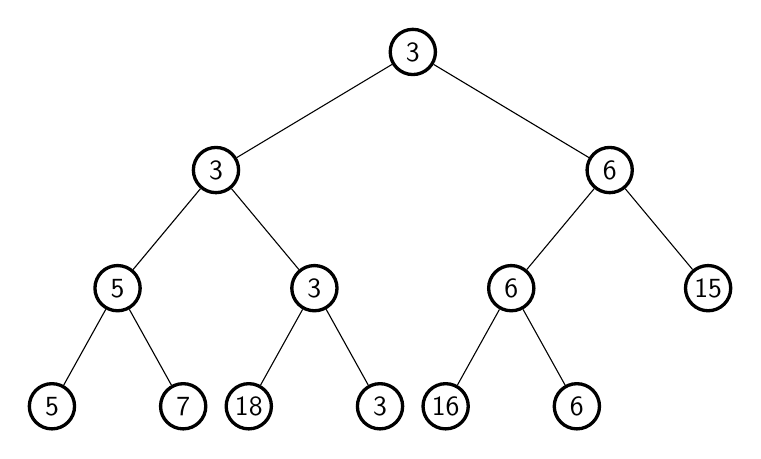
\begin{tikzpicture}[level/.style={sibling distance = 5cm/#1,
          level distance = 1.5cm}] 
        \node [treenode] {3}
            child{ 
                node [treenode] {3} 
                child{ 
                    node [treenode] {5} 
                	child{ 
                	    node [treenode] {5} 
                	}
        			child{
        			    node [treenode] {7}
        			}
                }
                child{ 
                    node [treenode] {3}
        			child{ 
        			    node [treenode] {18}
        			}
        			child{
        			    node [treenode] {3}
        			}
                }                            
            }
            child{ 
                node [treenode] {6}
                child{ 
                    node [treenode] {6} 
        			child{ 
        			    node [treenode] {16}
        			}
        			child{
        			    node [treenode] {6}
        			}
                }
                child{ 
                    node [treenode] {15}
                }
        	}
        ;
        \end{tikzpicture}
        \captionsetup{type=figure, width=.76\linewidth}
        \captionof{figure}{Segment tree for the sequence $5,7,18,3,16,6,15$. Each node contains the minimum value of the corresponding sequence.}
    \end{center}

\subsection{Construction}
The following procedure returns the Segment Tree root for the sequence $x$ of length $n=\mathit{size}(x)$:
    \begin{algorithmic}[1]
    \Procedure{Build}{$x$}
        \State $\mathit{root}\gets$\Call{Recursive\_build}{$x,0,size(x)-1$}
        \State \textbf{return} $root$
    \EndProcedure
    \State
    \Function{Recursive\_build}{$x,l,r$}
        \State $\mathit{tmp}\gets\text{new Segment Tree node}$
        \If{$l=r$}
            \State $\mathit{tmp.data}\gets x_l$
            \State $\mathit{tmp.left}\gets \mathit{null}$
            \State $\mathit{tmp.right}\gets \mathit{null}$
        \Else
            \State $\mathit{tmp.left}\gets$\Call{Recursive\_build}{$x,l,\left\lfloor{\frac{l+r}{2}}\right\rfloor$}
            \State $\mathit{tmp.right}\gets$\Call{Recursive\_build}{$x,\left\lfloor{\frac{l+r}{2}}\right\rfloor+1,r$}
            \State $\mathit{tmp.data}\gets\min\{\mathit{tmp.left.data},\mathit{tmp.right.data}\}$
        \EndIf
        \State \textbf{return} $\mathit{tmp}$
    \EndFunction
    \end{algorithmic}
For a sequence of length $n$ the number of nodes created is:
    \begin{align*}
        f(n)=
        \begin{cases}
            1 \qquad &n=1 \\
            1+f(\left\lfloor{\frac{n}{2}}\right\rfloor)+f(\left\lceil{\frac{n}{2}}\right\rceil) \qquad &n>1
        \end{cases}
    \end{align*}
it follows that $f(n)=\mathcal{O}(n)$ and since the function \texttt{Recursive\_build} is called once for each node, the complexity of the construction procedure is $\mathcal{O}(n)$. Also assuming that each element of the sequence has a value between $-M$ and $M$, the number of bits needed to contain the information of all nodes is $\mathcal{O}(n\log{2M})$.

\subsection{selectLast and selectFirst}
With this data structure it is possible to efficiently implement the query $\texttt{selectFirst}_x(i,v)$ after building the Segment Tree related to $x$ (whose root is \texttt{root}):
    \begin{algorithmic}[1]
    \Procedure{selectFirst}{$root,x,i,v$}
        \State \textbf{return} \Call{selectFirstRecursive}{$\mathit{root},i,v,0,\mathit{size}(x)-1$}
    \EndProcedure
    \State
    \Function{selectFirstRecursive}{$node,ind,val,l,r$}
        \If{$ind\geq r \lor node.data>val$}
            \State $res\gets -1$
        \ElsIf{$l=r$}
            \State $res\gets l$
        \Else
            \State $res\gets$\Call{selectFirstRecursive}{$node.left,ind,val,l,\left\lfloor{\frac{l+r}{2}}\right\rfloor$}
            \If{$res\neq -1$}
                \State $res\gets$\Call{selectFirstRecursive}{$node.right,ind,val,\left\lfloor{\frac{l+r}{2}}\right\rfloor+1,r$}
            \EndIf
        \EndIf
        \State \textbf{return} $res$
    \EndFunction
    \end{algorithmic}
The number of nodes visited and the complexity of this procedure is $\mathcal{O}(\log{n})$. In a similar way we can implement the procedure $\texttt{selectLast}_x(i,v)$:
    \begin{algorithmic}[1]
    \Procedure{selectLast}{$\mathit{root},x,i,v$}
        \State \textbf{return} \Call{selectLastRecursive}{$\mathit{root},i,v,0,\mathit{size}(x)-1$}
    \EndProcedure
    \State
    \Function{selectLastRecursive}{$\mathit{node},\mathit{ind},\mathit{val},l,r$}
        \If{$\mathit{ind}\leq l \lor \mathit{node.data}>\mathit{val}$}
            \State $\mathit{res}\gets -1$
        \ElsIf{$l=r$}
            \State $\mathit{res}\gets l$
        \Else
            \State $\mathit{res}\gets$\Call{selectLastRecursive}{$\mathit{node.right},\mathit{ind},\mathit{val},\left\lfloor{\frac{l+r}{2}}\right\rfloor+1,r$}
            \If{$\mathit{res}\neq -1$}
                \State $\mathit{res}\gets$\Call{selectLastRecursive}{$\mathit{node.left},\mathit{ind},\mathit{val},l,\left\lfloor{\frac{l+r}{2}}\right\rfloor$}
            \EndIf
        \EndIf
        \State \textbf{return} $\mathit{res}$
    \EndFunction
    \end{algorithmic}    
Note that we have efficiently implemented selectLast and selectFirst queries, but not succinctly (because building the Segment Tree for an entire list of integers require $\Omega(n)$ additional bits).
\section{Two level organization of the information}
Given a list $v$ of integers of length $n$, divide it into \textit{super blocks} of size $\log^2{n}$ (first level) and divide each super block into \textit{blocks} of size $\log{n}$ (second level) and let $k=\log{n}$. Assuming that each integers in the list have a value between $-M$ and $M$, this chapter will show a succinct two-level organization of the information.

\subsection{First Level}
The number of super blocks in this level is $\frac{n}{k^2}$ (numbered from $0$ to $\frac{n}{k^2}-1$), for each of them calculate the minimum rank present obtaining the sequence $S$:
    $$
    S_i = \min_{ik^2 \leq j < (i+1)k^2}\{\text{rank}_v(j)\} \qquad 0\leq i < \frac{n}{k^2}
    $$
Build a Segment Tree for this sequence: since the value of $\text{rank}_v(j)$ is between $-nM$ and $nM$ (because it is the rank value of a list of $n$ integers between $-M$ and $M$) and the sequence $S$ has length $\frac{n}{k^2}$, that Segment Tree will occupy $\mathcal{O}(\frac{n}{k^2}\log{(2nM+1)})=\mathcal{O}(\frac{n}{k^2}(\log{(n)}+\log{(2M)})=\mathcal{O}(\frac{n}{\log{(n)}})=o(n\log{(2M)})$ bits.

Then calculate the sequence $T$ composed of the initial rank of each super block:
    $$
    T_i = \text{rank}_v(ik^2) \qquad 0\leq i < \frac{n}{k^2}
    $$
if we store the sequence $T$ in an array the number of bits needed will also be $\frac{n}{k^2}\log{(2nM+1)}=o(n\log{(2M)})$, so the total number of bits used to store this first layer of information is $o(n\log{(2M)})$.

\subsection{Second Level}
The number of blocks in this level is $\frac{n}{k}$ (numbered from $0$ to $\frac{n}{k}-1$), for each of them calculate the minimum rank present as a difference to the initial rank of its super block:
    $$
    B_i = \left(\min_{ik \leq j < (i+1)k}\{\text{rank}_v(j)\}\right)-T_{\left\lfloor{\frac{i}{k}}\right\rfloor} \qquad 0\leq i < \frac{n}{k}
    $$
if we save the sequence $B$ in an array the number of bits needed is $\frac{n}{k}\log{(2\log^2{(n)}M+1)}=\frac{n}{\log{n}}\cdot\mathcal{O}(2\log{\log{n}}+\log{(2M)})=o(n\log{(2M)})$ because each element of $B$ will be between $-\log^2{(n)}M$ and $\log^2{(n)}M$.

Let's also calculate the sequence $A$ of the differences between the initial rank of each block and the initial rank of its super block:
    $$
    A_i = \text{rank}_v(ik)-T_{\left\lfloor{\frac{i}{k}}\right\rfloor} \qquad 0\leq i < \frac{n}{k}
    $$
if we save the sequence $A$ in an array the number of bits needed is $\frac{n}{k}\log{(2\log^2{(n)}M+1)}=o(n\log{(2M)})$, so in total the number of bits used to store this second layer of information is $o(n\log{(2M)})$.

\section{Succinct rank, selectFirst and selectLast}
Once built the Segment Tree $S$ (whose root will be indicated with \texttt{root}) and calculated the values of $T$, $B$ and $A$ (they can be computed in $\mathcal{O}(n)$) relative to the sequence of parentheses $v$ you can calculate
    $$\text{rank}_v(i) = T_{\left\lfloor{\frac{i}{k^2}}\right\rfloor}+A_{\left\lfloor{\frac{i}{k}}\right\rfloor}+\sum_{j=k(\left\lfloor{\frac{i}{k}}\right\rfloor)}^{i-1} v_j$$
in $\mathcal{O}(\log{n})$ (the summation contains at most $\log{n}$ addends). 
    \begin{algorithm}[H]
    \caption{\texttt{rank}}
    \begin{algorithmic}[1]
    \Procedure{rank}{$T,A,n,v,i$}\Comment{$\mathit{rank}_v(i)$}
        \State $k\gets\log{n}$
        \State $u\gets T_{\left\lfloor{\frac{i}{k^2}}\right\rfloor}+A_{\left\lfloor{\frac{i}{k}}\right\rfloor}$
        \For{$j\gets k(\left\lfloor{\frac{i}{k}}\right\rfloor)\ \textbf{to}\ i-1$}
            \State $u\gets u+v_j$
        \EndFor
        \State \textbf{return} $u$
    \EndProcedure
    \end{algorithmic}
    \end{algorithm}
Moreover you can perform the query \texttt{selectFirst(i,u)} as follows:
    \begin{enumerate}
        \item Calculate $\mathit{tmp} = \text{rank}_v(i)$ (as explained above)
        \item Check if the searched position belongs to the same block of the index $i$ by performing a linear scan of all integers following $i$ until the end of the block it belongs to ($v_{i+1},\dots,v_{k(\left\lfloor{\frac{i}{k}}\right\rfloor+1)-1}$): if there is an index $x$ such that $\mathit{tmp} + \sum_{y=i}^{x-1}v_y = \mathit{rank}_v(x) <= u$ then $x$ is the position searched for. During this process, there are at most $k=\log{n}$ accesses to the sequence $v$;
        \item Otherwise check if the searched position belongs to the same super block of the index $i$ by scanning the values of $B$ related to blocks after $i$ until the end of the super block that $i$ belongs to ($B_{\left\lfloor{\frac{i}{k}}\right\rfloor+1},\dots,B_{k(\left\lfloor{\frac{i}{k^2}}\right\rfloor+1)-1}$): if there is an index $x$ such that $B_x+T_{\left \lfloor{\frac{i}{k^2}}\right\rfloor} \leq u$ then the searched position belongs to the block $x$ (and this block is in the same super block of the index $i$), in this case to find the exact position in the block is sufficient a scan of all the integers in that block ($v_{xk},v_{xk+1},\dots,v_{xk+k-1}$) until the first index $y$ such that $\mathit{rank}_v(y) \leq u$ (note how you can calculate the value of $\mathit{rank}_v(y)$ during the scan using the same formula of step $2$). During this process, there are at most $k=\log{n}$ accesses to the sequence $B$ and at most $k=\log{n}$ accesses to the sequence $v$;
        \item If the position was not found after the steps $2$ and $3$ means that the searched position is in another super block than the one where $i$ is, to find that super block just call the procedure \texttt{selectFirst}$(\mathit{root},S,\left\lfloor{\frac{i}{k^2}}\right\rfloor,u)$ that will return the index $x$ of the first super block that follows $i$ containing an excess less than or equal to $u$. At that point you have to search for the block where the searched position is located and then search for the exact position in a similar way as explained in step $3$: scan the values of $B$ relative to the blocks contained in the super block $x$ ($B_{xk},\dots,B_{xk+k-1}$) and if there is an index $y$ such that $B_y+T_x \leq u$ then the searched position is in the block $y$, finally to find the exact index you need to scan all the integers of that block ($v_{yk},\dots,v_{yk+k-1}$) until you find the first index $z$ such that $\mathit{rank}_v(z) \leq u$. During this process a call is made to the function \texttt{selectFirst}$(\mathit{root},S,\left\lfloor{\frac{i}{k^2}}\right\rfloor,u)$ (which has complexity $\mathcal{O}(\log{\frac{n}{k^2}})=\mathcal{O}(\log{n})$) and there are at most $k=\log{n}$ accesses to the sequence $B$ and at most $k=\log{n}$ accesses to the sequence $v$;
    \end{enumerate}

In conclusion you can implement succinctly the \texttt{selectFirst} query with complexity $\mathcal{O}(\log{n})$ using the sequence $v$ of integers that occupies $n\log{(2M+1)}$ bits and other auxiliary structures (the Segment Tree related to the sequence $S$ and the sequences $T,B,A$) that occupy $o(n\log{(2M)})$ bits. The following pseudocode shows the implementation of the whole procedure:
    \begin{algorithm}
    \caption{\texttt{selectFirst}}\label{selectFirst} 
    \begin{algorithmic}[1]
    \Procedure{selectFirst}{$\mathit{root},S,T,B,A,n,v,i,u$} \Comment{$\mathit{selectFirst}_v(i,u)$}
        \State $k\gets\log{n}$
        \State $\mathit{tmp} \gets \Call{rank}{T,A,n,v,i}$ \Comment{step 1}
        \State
        \For{$x\gets i+1\ \textbf{to}\ k(\left\lfloor{\frac{i}{k}}\right\rfloor+1)-1$} \Comment{step 2}
            \State $\mathit{tmp}\gets \mathit{tmp}+v_{x-1}$
            \If{$\mathit{tmp}\leq u$}
                \State \textbf{return} $x$
            \EndIf
        \EndFor
        \State
        \For{$x\gets \left\lfloor{\frac{i}{k}}\right\rfloor+1\ \textbf{to}\ k(\left\lfloor{\frac{i}{k^2}}\right\rfloor+1)-1$}\Comment{step 3}
            \If{$B_x+T_{\left\lfloor{\frac{i}{k^2}}\right\rfloor} \leq u$}
                \State $\mathit{currt}\gets T_{\left\lfloor{\frac{i}{k^2}}\right\rfloor}+A_x$
                \For{$y\gets xk\ \textbf{to}\ xk+k-1$}
                    \If{$\mathit{currt} \leq u$}
                        \State \textbf{return} $y$
                    \EndIf
                    \State $\mathit{currt}\gets \mathit{currt}+v_y$
                \EndFor
            \EndIf
        \EndFor
        \State
        \State $x\gets \Call{Find\_succ}{\mathit{root},S,\left\lfloor{\frac{i}{k^2}}\right\rfloor,u}$ \Comment{step 4}
    \algstore{alg1}            
    \end{algorithmic}
    \end{algorithm}
    \begin{algorithm}
    \begin{algorithmic}[1]
    \algrestore{alg1}
        \If{$x\neq -1$}
            \For{$y\gets xk\ \textbf{to}\ xk+k-1$}
                \If{$B_y+T_x \leq u$}
                    \State $\mathit{currt}\gets T_x+A_y$
                    \For{$z\gets yk\ \textbf{to}\ yk+k-1$}
                        \If{$\mathit{currt} \leq u$}
                            \State \textbf{return} $z$
                        \EndIf
                        \State $\mathit{currt}\gets \mathit{currt}+v_z$
                    \EndFor
                \EndIf
            \EndFor
        \EndIf
        \State \textbf{return} $-1$ \Comment{there is no such index}
    \EndProcedure
    \end{algorithmic}
    \end{algorithm}
    
Symmetrically you can implement the operation \texttt{selectLast(i,u)}: initially we check if the searched position is in the same block of $i$, otherwise we check if it is present in the same super block of $i$ and otherwise we search for the correct super block, the correct block within the super block and finally the exact position within the block:
    \begin{algorithm}[H]
    \caption{\texttt{selectLast}}\label{selectLast} %sei arrivato fino a qua
    \begin{algorithmic}[1]
    \Procedure{selectLast}{$\mathit{root},S,T,A,B,n,v,i,u$}\Comment{$\mathit{selectLast}_v(i,u)$}
        \State $k\gets\log{n}$
        \State $\mathit{tmp}\gets\Call{rank}{T,A,n,v,i}$\Comment{step 1}
        \State
        \For{$x\gets i-1\ \textbf{down to}\ k\left\lfloor{\frac{i}{k}}\right\rfloor$}\Comment{step 2}
            \State $\mathit{tmp}\gets \mathit{tmp}-v_x$
            \If{$\mathit{tmp} \leq u$}
                \State \textbf{return} $x$
            \EndIf
        \EndFor
        \State
        \For{$x\gets \left\lfloor{\frac{i}{k}}\right\rfloor-1\ \textbf{down to}\ k(\left\lfloor{\frac{i}{k^2}}\right\rfloor)$}\Comment{step 3}
            \If{$B_x+T_{\left\lfloor{\frac{i}{k^2}}\right\rfloor} \leq u$}
                \State $\mathit{currt}\gets T_{\left\lfloor{\frac{i}{k^2}}\right\rfloor}+A_{x+1}$
                \For{$y\gets xk+k-1\ \textbf{down to}\ xk$}
                    \State $\mathit{currt}\gets \mathit{currt}-v_y$
                    \If{$\mathit{currt} \leq u$}
                        \State \textbf{return} $y$
                    \EndIf
                \EndFor
            \EndIf
        \EndFor
        \State
        \State $x\gets \Call{selectLast}{\mathit{root},S,\left\lfloor{\frac{i}{k^2}}\right\rfloor,u}$ \Comment{step 4}
        \If{$x \neq -1$}
            \For{$y\gets xk+k-1\ \textbf{down to}\ xk$}
                \If{$B_y+T_x \leq u$}
                    \If{$y<xk+k-1$}
                        \State $\mathit{currt}\gets T_x+A_{y+1}$
                    \Else
                        \State $\mathit{currt}\gets T_{x+1}$
                    \EndIf
                    \For{$z\gets yk+k-1\ \textbf{down to}\ yk$}
                        \State $\mathit{currt}\gets \mathit{currt}-v_z$
                        \If{$\mathit{currt} \leq u$}
                            \State \textbf{return} $z$
                        \EndIf
    \algstore{alg1}            
    \end{algorithmic}
    \end{algorithm}
    \begin{algorithm}[ht]
    \begin{algorithmic}[1]
    \algrestore{alg1}
                    \EndFor
                \EndIf
            \EndFor
        \EndIf
        \State \textbf{return} $-1$ \Comment{there is no such index}
    \EndProcedure
    \end{algorithmic}
    \end{algorithm}

\section{An application of generalized rank/select queries: sequences of balanced parenthesis}
A sequence $V$ of parentheses is balanced if in each prefix of $V$ the number of open parentheses is greater than or equal to the number of closed parentheses, and the total number of open parentheses in $V$ is equal to the number of closed parentheses. In a less formal way it can be defined as a sequence of parentheses from which a valid arithmetic operation can be obtained by adding some numbers and operations. Some useful operations on such sequences are the following:
    \begin{itemize}
    \item \texttt{find\_close(i)}: given an open parenthesis with index $i$, calculate the index of the corresponding closed parenthesis;
    \item \texttt{find\_open(i)}: given a closed parenthesis with index $i$, calculate the index of the corresponding open parenthesis;
    \item \texttt{find\_enclose(i)}: given a parenthesis with index $i$, calculate the positions $(x,y)$ of matching parentheses enclosing it. If there are multiple pairs with this property, select the innermost one, that is the one that does not contain other valid pairs (for a more formal definition read the \textbf{Notations}). 
    \end{itemize}
This chapter will show how, given a balanced parentheses sequence of length $2n$, to perform such operations with a time complexity of $\mathcal{O}(\log{n})$ using $2n + o(n)$ bits of memory.

\subsection{Notations}
Let $v$ be a sequence of parentheses of length $2n$ numbered from $0$ to $2n-1$ and $v_i$ the parenthesis with index $i$. For convenience, assume a value of $v_i=1$ indicates an open parenthesis at position $i$ and a value of $v_i=-1$ indicates a closed parenthesis at position of $i$. We define the excess of a position $i$ as:
    $$
    \mathit{excess}_v(i) = |\{j :\ j<i \land v_i=1\}|-|\{j :\ j\leq i \land v_i=-1\}|
    $$
that is the difference between the number of open parentheses preceding $i$ (excluded) and the number of closed parentheses preceding $i$ (included).
It follows that a sequence of parentheses is balanced if and only if:
    \begin{align*}
    \mathit{excess}_v(i) &\geq 0 \qquad 0\leq i < 2n-1 \\
    \mathit{excess}_v(2n-1) &= 0
    \end{align*}
It also follows the definition of the operations of $\text{find\_close}, \text{find\_open}$ and $\text{find\_enclose}$:
    \begin{align*}
    \mathit{findClose}_v(i) &= 
        \begin{cases}
            \min\{j :\ j>i \land \mathit{excess}_v(j)=\mathit{excess}_v(i)\} \qquad &v_i = 1 \\
            -1 \qquad &v_i = -1
        \end{cases} \\
    \mathit{findOpen}_v(i) &= 
        \begin{cases}
            \max\{j :\ j<i \land \mathit{excess}_v(j)=\mathit{excess}_v(i)\} \qquad &v_i = -1 \\
            -1 \qquad &v_i = 1
        \end{cases}\\
    \mathit{leftEnclose}_v(i) &= 
        \begin{cases}
        \max\{j :\ j<i \land \mathit{excess}_v(j)+1=\mathit{excess}_v(i)\} \qquad &\mathit{excess}_v(i) > 0 \\
        -1 \qquad &\mathit{excess}_v(i) = 0
        \end{cases}\\
    \mathit{rightEnclose}_v(i) &=
    \begin{cases}
    \min\{j :\ j>i \land \mathit{excess}_v(j)+1=\mathit{excess}_v(i)\} \qquad &\mathit{excess}_v(i) > 0 \\
    -1 \qquad & \mathit{excess}_v(i) = 0
    \end{cases}\\
    \mathit{findEnclose}_v(i) &= (\mathit{leftEnclose}_v(i),\mathit{rightEnclose}_v(i))
    \end{align*}
Note how $\mathit{findClose}(i)$ will always return the index of a closed parentheses (assuming $v$ is a sequence of balanced parenthesis and $v_i=1$) and $\mathit{findOpen}(i)$ will always return the index of an open parentheses (assuming $v$ is a sequence of balanced parenthesis and $v_i=-1$).

Finally let $S,T,B,A$ be the two-level organization of the information relative to the sequence $v$, the total number of additional bits required will be $o(n\log{3})=o(n)$ because $v$ contain only $\pm 1$ values.

\subsection{Excess}
If we consider an open parentheses as $+1$ and a closed parentheses as $-1$, the excess of a position $i$ will be:
     \begin{align*}
        \mathit{excess}_v(i)=
        \begin{cases}
            \sum_{j=0}^{i-1}v_j = \mathit{rank}_v(i) \qquad &v_i=1 \\
            \sum_{j=0}^{i}v_j = \mathit{rank}_v(i)-1 \qquad &v_i=-1
        \end{cases}
    \end{align*}
therefore it can be calculated with complexity $\mathcal{O}(\log{n})$ (due to the single rank query).

\subsection{FindClose and findOpen}
Let $a$ be the index of an open parenthesis ($v_a = 1$), $u = \mathit{excess}_v(a) = \mathit{rank}_v(a)$ and $b = \mathit{findClose}_v(a)$ (note that $v_b=-1$). If $v$ is a sequence of balanced parentheses then $v_{a+1},v_{a+2},\dots,v_{b-1}$ will also be a sequence of balanced parentheses and
    \begin{align*}
        \sum_{i=a+1}^{x} v_i &\geq 0 \qquad \forall a+1 \leq x \leq b-2 \\
        \sum_{i=a+1}^{b-1} v_i &= 0.
    \end{align*}
It follows that
    \begin{align*}
        \mathit{rank}_v(x) &= \mathit{rank}_v(a)+v_a+\sum_{i=a+1}^{x-1} v_i > \mathit{rank}_v(a) \qquad \forall a+2 \leq x \leq b \\
        \mathit{rank}_v(b+1) &= \mathit{rank}_v(a)+v_a+\sum_{i=a+1}^{b-1} v_i+v_b = \mathit{rank}_v(a) + 1 + 0 - 1 = \mathit{rank}_v(a)
    \end{align*}
and $b+1$ is the first index $x$ greater than $a$ such that $\mathit{rank}_v(x) \leq \mathit{rank}_v(a)$. As a result
    \begin{align*}
        b+1 &= selectFirst_v(a,\mathit{rank}_v(a)) \\
        \mathit{findClose}_v(a) &= \mathit{selectFirst}_v(a,\mathit{rank}_v(a)) - 1=\mathit{selectFirst}_v(a,\mathit{excess}_v(a)) - 1.
    \end{align*}
Similarly it is possible to prove that if $a$ is the index of a closed parentheses ($v_a = -1$) then $\mathit{findOpen}_v(a)=\mathit{selectLast}_v(a,\mathit{rank}_v(a)-1)$. Let $u = \mathit{excess}_v(a) = \mathit{rank}_v(a) - 1$ and $b = \mathit{findOpen}_v(a)$ (note that $v_b=1$), if $v$ is a sequence of balanced parentheses then $v_{b+1},v_{b+1},\dots,v_{a-1}$ will also be a sequence of balanced parentheses and
     \begin{align*}
        \sum_{i=x}^{a-1} v_i &\leq 0 \qquad \forall b+2 \leq x \leq a-1 \\
        \sum_{i=b+1}^{a-1} v_i &= 0.
    \end{align*}
It follows that
    \begin{align*}
        \mathit{rank}_v(x) &= \mathit{rank}_v(a)-\sum_{i=x}^{a-1} v_i \geq \mathit{rank}_v(a) > \mathit{rank}_v(a)-1 \qquad \forall a+1 \leq x \leq b \\
        \mathit{rank}_v(b) &= \mathit{rank}_v(a)-\sum_{i=a+1}^{b-1}v_i-v_b = \mathit{rank}_v(a) - 0 - 1 = \mathit{rank}_v(a) - 1
    \end{align*}
and $b$ is the last index $x$ less than $a$ such that $\mathit{rank}_v(x) \leq \mathit{rank}_v(a) - 1$. As a result
    \begin{align*}
        b &= selectLast_v(a,\mathit{rank}_v(a)-1) \\
        \mathit{findClose}_v(a) &= \mathit{selectLast}_v(a,\mathit{rank}_v(a)-1)=\mathit{selectLast}_v(a,\mathit{excess}_v(a)).
    \end{align*}
    
\subsection{LeftEnclose and rightEnclose}
The operation $\mathit{leftEnclose}_v(i)$ is analogous to $\mathit{findOpen}_v(i)$ with the only difference that the excess searched is not $\mathit{excess}_v(i)$ but $\mathit{excess}_v(i)-1$ (and there is no solution if $\mathit{excess}_v(i)=0$):
    \begin{align*}
        \mathit{leftEnclose}_v(i) =
        \begin{cases}
            \mathit{selectLast}_v(i,\mathit{excess}_v(i)-1) \qquad &\mathit{excess}_v(i)>0 \\
            -1 \qquad &\mathit{excess}_v(i)=0
        \end{cases}
    \end{align*}
And similarly the operation \texttt{rightEnclose} is analogous to $\mathit{findClose}_v(i)$ with the only difference that the excess searched is not $\mathit{excess}_v(i)$ but $\mathit{excess}_v(i)-1$ (and there is no solution if $\mathit{excess}_v(i)=0$): 
    \begin{align*}
        \mathit{rightEnclose}_v(i) =
        \begin{cases}
            \mathit{selectFirst}_v(i,\mathit{excess}_v(i)-1) \qquad &\mathit{excess}_v(i)>0 \\
            -1 \qquad &\mathit{excess}_v(i)=0
        \end{cases}
    \end{align*}
    
\section{Experiments}

\subsection{succinctRankSelectDS}
The name succinctRankSelectDS refers to the data structure described in Chapters 3 and 4 that allows rank, selectFirst, and selectLast queries to be performed on lists of integers in a succinct manner (as explained in Chapter 5). In this chapter we will talk about the implementation in Golang of this data structure, a correctness test and its comparison with the Jacobson structure regarding the rank query (on bit sequences).

\subsubsection{Correctness test of the implementation}
It was decided to structure the test according to the following parameters:
    \begin{itemize}
       \item $t$ (number of tests): the number of integer lists to be generated and tested;
        \item $n$ (sequence size):  the number of integers in each sequence;
        \item $M$ (value size): $M-1$ is the maximum value that can assume the absolute value of each integer;
        \item $q$ (queries size): the number of queries that will be made on each sequence.
    \end{itemize}
Each query is generated with uniform probability between $\mathit{rank}_v(i)$, $\mathit{selectLast}_v(i,u)$, $\mathit{selectFirst}_v(i,u)$ and $\mathit{select}_v(u)$ (which is equivalent to a $\mathit{select}_v(i,u)$ with $i=n-1$). Each index $i$ used in queries is generated with uniform probability between $0$ and $n-1$ while any value $u$ used is generated with uniform probability between $-n(M-1)$ and $n(M-1)$. Instead, for the lists to query, each of the $t$ lists is randomly generated by assigning each element with uniform probability a value between $-M+1$ and $M-1$, this way each of the possible $(2M-1)n$ lists of integers has the same probability of being generated.

The results of each query are compared to those obtained by slowRankSelectDS, a data structure that performs rank/select operations in a naive $\mathcal{O}(n)$ complexity by linearly scanning the list of integers to answer each query.

\subsubsection{Comparison with JacobsonDS}
The name SlowJacobsonDS refers the classic implementation of Jacobson’s rank for bit sequences. The rank query has complexity $\mathcal{O}(\log{n})$ because to get the index of the table to be queried in the second level of the structure a portion of the array is scanned linearly ad will be scanned at most $\frac{1}{2}\log{n} = \mathcal{O}(\log{n})$ bits. The name JacobsonDS instead refers the implementation of Jacobson's rank where the computation of the index of the table to be queried uses a constant number of bitwise operations (to extrapolate portions of bits with a single operation) and then the rank will have complexity $\mathcal{O}(1)$, but note that in order to achieve such complexity it is necessary that the number of bits to access to establish the table index to be queried in the second level, that is $\frac{1}{2}\log{n}$, is equal to $\mathcal{O}(W)$, where $W$ is the wordsize of the computing machine.

The bit sequences on which to operate were generated randomly by assigning a random value to each bit, always with uniform probability so that each bits sequence of length $n$ is equiprobable. The generated indexes that will be used by rank queries are $30\cdot 10^6$, grouped in $30$ groups of $10^6$, and were generated with uniform probability between $0$ and $n-1$. For each group of indexes the average rank time for each of the three data structures has been calculated using the Go time package.

\begin{center}
    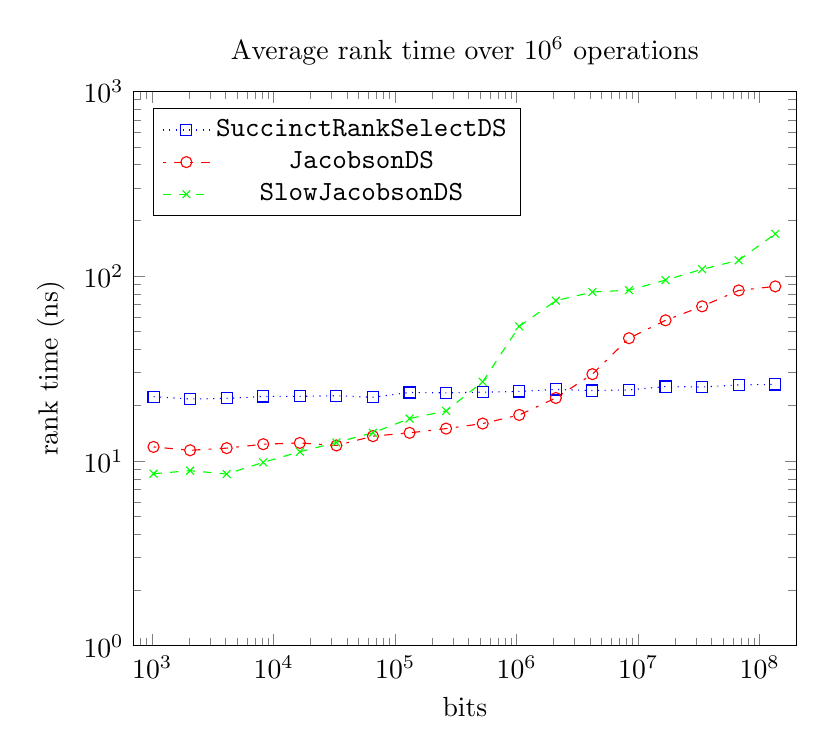
\begin{tikzpicture}
    \begin{axis}[
        title={Average rank time over $10^6$ operations},
        xmode=log,
        ymode=log,
        xlabel={bits},
        ylabel={rank time (ns)},
        xmin=700, xmax=200000000,
        ymin=1, ymax=1000,
        legend pos=north west,
        grid style=dashed
        %legend style={font=\tiny}
    ]
    
    \addplot[
        color=blue,
        dotted,
        mark=square,
        mark options={solid}
        ]
        coordinates {
        (1024,22.260389866666664)(2048,21.632234499999996)(4096,21.78527973333333)(8192,22.31620623333334)(16384,22.3508161)(32768,22.518472633333335)(65536,22.106238166666667)(131072,23.44986696666667)(262144,23.3546266)(524288,23.54799120000001)(1048576,23.766337966666672)(2097152,24.356845)(4194304,24.020421400000007)(8388608,24.216382266666663)(16777216,25.253238599999996)(33554432,25.112168766666663)(67108864,25.771720966666667)(134217728,25.925554166666675)
        };
        \addlegendentry{\texttt{SuccinctRankSelectDS}}
        
    \addplot[
        color=red,
        dash pattern=on 1pt off 3pt on 3pt off 3pt,
        mark=o,
        mark options={solid}
        ]
        coordinates {
        (1024,11.9079315)(2048,11.415417066666667)(4096,11.726542933333336)(8192,12.315543966666668)(16384,12.5096618)(32768,12.124949866666665)(65536,13.612070033333334)(131072,14.185817066666669)(262144,14.9554078)(524288,15.927701266666666)(1048576,17.7290944)(2097152,21.90122986666666)(4194304,29.475657366666663)(8388608,46.112946266666654)(16777216,57.614466033333315)(33554432,68.56925756666666)(67108864,83.6088405)(134217728,87.92505726666666)
        };
        \addlegendentry{\texttt{JacobsonDS}}
        
    \addplot[
        color=green,
        dashed,
        mark=x,
        mark options={solid}
        ]
        coordinates {
        (1024,8.527320333333334)(2048,8.8580143)(4096,8.495861933333334)(8192,9.826865733333335)(16384,11.2087367)(32768,12.587983633333328)(65536,14.196538933333333)(131072,16.954471666666667)(262144,18.637653066666665)(524288,26.79197683333333)(1048576,53.48165106666667)(2097152,73.59647573333334)(4194304,81.9556144333333)(8388608,83.87903903333333)(16777216,95.09200526666665)(33554432,108.8487699)(67108864,121.6854127)(134217728,169.19223623333335)
        };
        \addlegendentry{\texttt{SlowJacobsonDS}}
    \end{axis}
    \end{tikzpicture}
    \captionsetup{type=figure, width=.76\linewidth}
    \captionof{figure}{Comparison result for SuccinctRankSelectDS, JacobsonDS and SlowJacobsonDS}
\end{center}

As you can see for a reduced number of bits the most efficient data structure is SlowJacobsonDS because in that case the linear scan is faster than the cost of operations, albeit constant, necessary to extrapolate the indexes with JacobsonDS. As bits increase, the more efficient data structure becomes JacobsonDS because SlowJacobsonDS' linear scanning starts to become expensive while JacobsonDS keeps the number of operations constant. Finally, by further increasing the number of bits there is a drop in performance of both JacobsonDS and SlowJacobsonDS, probably due to the costs of access to the tables of the second level, while SuccinctRankSelectDS remains stable and then becomes the most performing one.

\begin{center}
    \begin{tabular}{ r | c | c | c }
        Size & \texttt{SuccinctRankSelectDS} & \texttt{JacobsonDS} & \texttt{SlowJacobsonDS} \\ \hline
        1 Kib & 22.26 & 11.91 & 8.53 \\
        16 Kib & 22.35 & 12.51 & 11.21 \\
        256 Kib & 23.35 & 14.96 & 18.64 \\
        4 Mib & 24.02 & 29.48 & 81.96 \\
        64 Mib & 25.77 & 83.61 & 121.69 \\
        128 Mib & 25.93 & 87.93 & 169.19 \\
    \end{tabular}
     \captionsetup{type=table, width=.76\linewidth}
    \captionof{table}{}
\end{center}

\subsection{SuccinctDS}
The name succintDS refers the data structure that implements the management of sequences of balanced parentheses as described in Chapter 6. A correctness test has also been carried out in this case.


\subsubsection{Random generation of sequences of balanced parentheses}
In order to perform a correctness test it is necessary to have generator of sequences of balanced parentheses. An ideal generator must return, given in input an integer $n$, any sequence of balanced parentheses of legnth $2n$ in a equiprobably way.

A well-known fact is that the number of sequence of balanced parentheses of length $2n$ is equal to the Catalan number $C(n) = \frac{1}{n+1}\binom{2n}{n}$. You can also have a one-to-one match between the sequences of balanced parentheses with length $2n$ and the paths in a $n\times n$ grid starting at the bottom-left corner $(0.0)$, ending at the top-right corner $(n,n)$, always moving to the right or up and never exceeding the main diagonal of equation $x=y$.

\begin{center}
    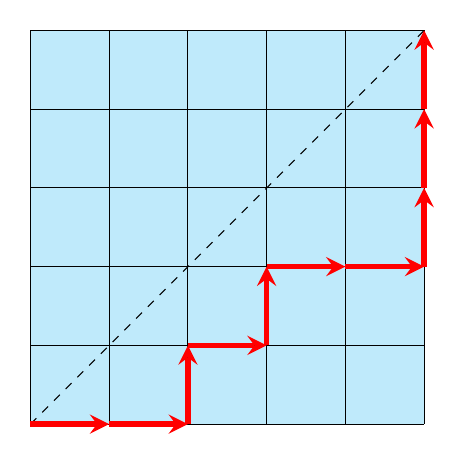
\begin{tikzpicture}
    \catalannumber{5}{5}{0,0,1,0,1,0,0,1,1,1}{0};
    \end{tikzpicture}
    \captionsetup{type=figure, width=.76\linewidth}
    \captionof{figure}{Path associated with the sequence of balanced parentheses (()()(()))}
    \label{ok1}
\end{center}
As you can see from the figure \ref{ok1}, if you associate an open parenthesis to an x-coordinate increment of the path and a closed parenthesis to a y-coordinate increment of the path, each sequence of balanced parentheses is associated with one and only one path. In addition, to be a sequence of balanced parentheses it is necessary that the number of open parenthesis in each prefix is always greater than or equal to the number of closed parenthesis, so the number of x-coordinate increments must always be greater than or equal to the number of y-coordinate increments. It follows that the path obtained will always be below the main diagonal, moreover each path that does not exceed the diagonal is associated with one and only one sequence ofbalanced parentheses.

\begin{center}
    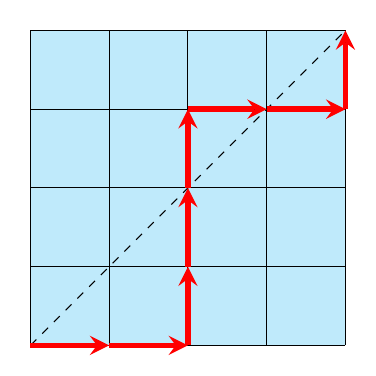
\begin{tikzpicture}
    \catalannumber{4}{4}{0,0,1,1,1,0,0,1}{0};
    \end{tikzpicture} 
    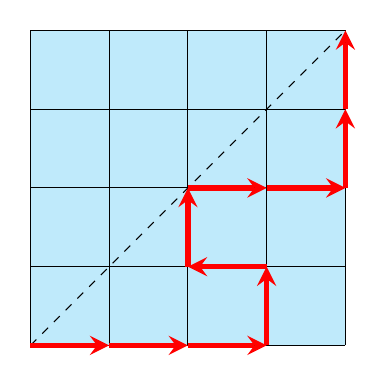
\begin{tikzpicture}
    \catalannumber{4}{4}{0,0,0,1,2,1,0,0,1,1}{0};
    \end{tikzpicture} 
    \captionsetup{type=figure, width=.76\linewidth}
    \captionof{figure}{Examples of invalid paths (the first one crosses the diagonal, the second one does not always go to the right or up but also goes to the left)}
\end{center}
Now suppose $N$ is a fixed integer, you have a prefix of $S$ of a sequence of balanced parentheses of length $2N$ and that this prefix has $K$ open parentheses more than the number of closed parentheses. Let $|S|$ be the number of parentheses contained in $S$ (which will then have $\frac{|S|+K}{2}$ open parentheses and $\frac{|S|-K}{2}$ closed parentheses) and $f(K)$ the number of parentheses sequences $T$ such that the concatenation $S+T$ is a sequence of balanced parentheses of length $2N$ ($T$ in particular does not have to be balanced, it will be so if and only if $K=0$). The value $f(K)$ searched is equal to the number of parentheses sequences of length $2N-|S|$ containing $\frac{2N-|S|-K}{2}$ open parentheses, $\frac{2N-|S|+K}{2}$ closed parentheses and such that in each prefix there are at most $K$ closed parentheses more than the number of open parentheses. Considering the one-to-one match explained above, it is equivalent to the number of paths in a $\frac{2N-|S|-K}{2} \times \frac{2N-|S|+K}{2}$ grid starting in $(0,0)$, ending in $(\frac{2N-|S|-K}{2},\frac{2N-|S|K}{2})$, that always go to the right or to up and never exceed the diagonal $y=x+K$.
\begin{center}
    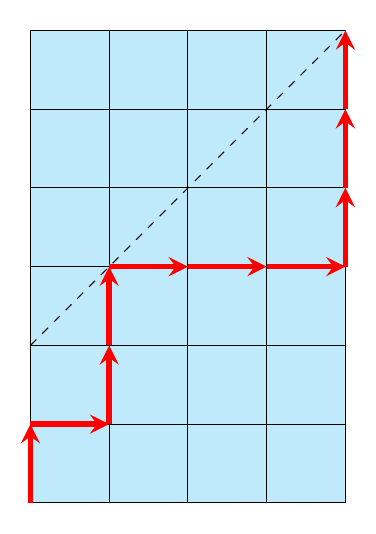
\begin{tikzpicture}
        \catalannumber{6}{4}{1,0,1,1,0,0,0,1,1,1}{2}
    \end{tikzpicture}
    \captionsetup{type=figure, width=.76\linewidth}
    \captionof{figure}{If $N=4,S=(($, the number of strings $T$ such that $S+T$ is balanced is equal to the number of paths going from $(0,0)$ to $(4,6)$ without exceeding the diagonal $y=x+2$. The red path matches the sequence $T=)())((()))$}
\end{center}
One way to count the number of such paths is as follows: you calculate the number of paths that exceed the diagonal and subtract it from the number of total paths, this same method is one of the ways to calculate Catalan numbers. To calculate the number of paths in a grid $A \times B$ that exceed the diagonal $y=x+K$ you may notice that if you take a path that exceeds the diagonal and reverse all moves after the first crossing of the diagonal (x-coordinate increments become y-coordinate increments and vice versa), you get a path that starts in $(0,0)$ and ends in $(A-K-1,A+B-(A-K)+1)$. In this way there is a one-to-one match between the number of paths that exceed the diagonal and the number of paths from $(0,0)$ to $(A-K-1,A+B-(A-K)+1)$
\begin{center}
\begin{tabular}{ccc}
    \begin{tabular}{l}
    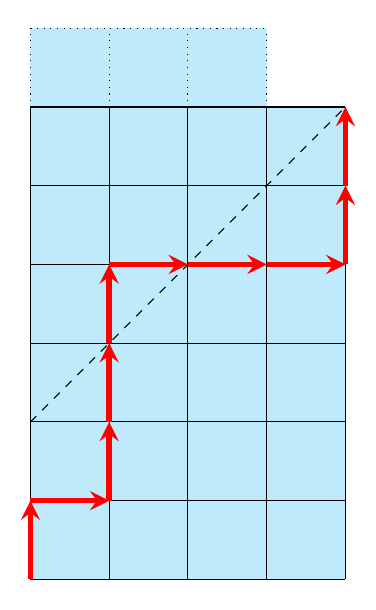
\begin{tikzpicture}
        \catalannumberextended{6}{4}{1,0,1,1,1,0,0,0,1,1}{2}
    \end{tikzpicture}
    \end{tabular} 
    &
    $\longrightarrow$ 
    &
    \begin{tabular}{l}
    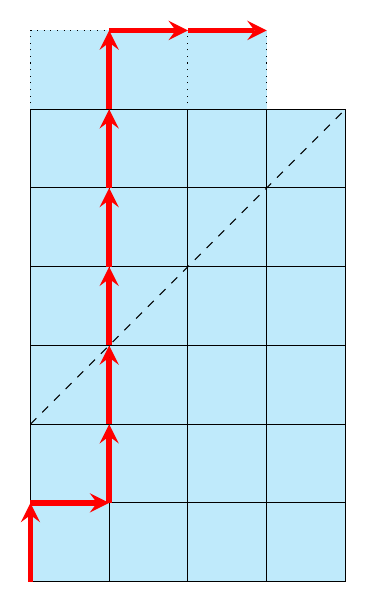
\begin{tikzpicture}
        \catalannumberextended{6}{4}{1,0,1,1,1,1,1,1,0,0}{2}
    \end{tikzpicture}
    \end{tabular}
\end{tabular}
\captionsetup{type=figure, width=.76\linewidth}
\captionof{figure}{If $A=6,B=4,K=2$, reversing each move after the first crossing of the diagonal gives a path from $(0,0)$ to $(3,7)$}
\end{center}
It follows that the number of paths in a $A\times B$ grid that do not exceed the diagonal $y=x+K$ is equal to the number of paths from $(0,0)$ to $(A,B)$ minus the number of paths from $(0,0)$ to $(A-K-1,A+B-(A-K)+1)$ which is equal to $\binom{A+B}{A}-\binom{A+B}{A-K-1}$. In particular with $A=B$ and $K=0$ you get the Catalan number $C(n)$.

Then to generate a sequence of balanced parentheses of length $2N$ the generator will start initially from an empty prefix, then until the length of the current prefix $S$ is less than $2N$ it will calculate the number $A$ of ways in which you can finish the prefix $S+($ and the number $B$ of ways in which you can end the prefix $S+)$ and choose to add an open or closed parentheses directly proportionally to those values, meaning with probability $\frac{A}{A+B}$ it will add an open parentheses and with probability $\frac{B}{A+B}$ will add a closed parenthesis. This way each sequence of balanced parentheses of legnth $2N$ will be equiprobable.

\subsubsection{Correctness test of the implementation}
The test was structured according to the following parameters:
    \begin{itemize}
        \item $t$ (number of tests): the number of integer sequences of balanced parentheses to be generated and tested;
        \item $n$ (sequence size): the number of parentheses pairs in each sequence;
        \item $q$ (queries size): the number of queries that will be made on each sequence of parentheses; 
    \end{itemize}
Each query is randomly generated with uniform probability between $\mathit{findClose}_v(i)$, $\mathit{findOpen}_v(i)$, $\mathit{findClose}_v(i)$ and $\mathit{findEnclose}_v(i)$. After generating $t$ sequences of balanced parentheses of $2n$ length using what is described in Chapter $\textbf{7.2.1}$, the results of the queries were compared with those obtained by slowDS, a non-succinct data structure that performs the operations $\mathit{findClose}_v(i)$, $\mathit{findOpen}_v(i)$, $\mathit{findClose}_v(i)$ and  $\mathit{findEnclose}_v(i)$ with linear complexity by scanning the parentheses sequence to answer each query.

\section{Conclusions}
It has been shown a data structure that allows to perform generalized rank/select queries on lists of $N$ integers (each between $-M$ and $M$) with $\mathcal{O}(\log{n})$ complexity using $N\log{(2M+1)}+o(N\log{M})$ bits. The initial construction of all necessary structures has complexity $\mathcal{O}(N)$. It has also been shown how it is possible to use this succinct structure for the management of sequences of balanced parentheses.

\end{document}
